\documentclass[letterpaper,11pt]{article}

\setlength{\voffset}{0.1in}
\setlength{\paperwidth}{8.5in}
\setlength{\paperheight}{11in}
\setlength{\headheight}{0in}
\setlength{\headsep}{0in}
\setlength{\textheight}{11in}
\setlength{\textheight}{9.5in}
\setlength{\topmargin}{-0.25in}
\setlength{\textwidth}{7in}
\setlength{\topskip}{0in}
\setlength{\oddsidemargin}{-0.25in}
\setlength{\evensidemargin}{-0.25in}

\usepackage{xunicode}
\usepackage{xltxtra}
\XeTeXlinebreaklocale "zh"
\XeTeXlinebreakskip = 0pt plus 1pt
\setsansfont{AR PL UKai CN}
\setromanfont{AR PL UKai CN}

%\usepackage{fullpage}
\usepackage{shading}
%\textheight=9.0in
\pagestyle{empty}
\raggedbottom
\raggedright
\setlength{\tabcolsep}{0in}
\usepackage{sphinx1}
\usepackage{picins}
\usepackage{graphicx}
%-----------------------------------------------------------
%Custom commands
\newcommand{\resitem}[1]{\item #1 \vspace{2pt}}
\newcommand{\resheading}[1]{{\large \parashade[.9]{sharpcorners}{\textbf{#1 \vphantom{p\^{E}}}}}}
\newcommand{\ressubheading}[4]{
\begin{tabular*}{6.5in}{l@{\extracolsep{\fill}}r}
        \textbf{#1} & #2 \\
        \textit{#3} & \textit{#4} \\
\end{tabular*}\vspace{2pt}}
%-----------------------------------------------------------


\usepackage{paralist}

\let\itemize\compactitem
\let\enditemize\endcompactitem
\let\enumerate\compactenum
\let\endenumerate\endcompactenum
\let\description\compactdesc
\let\enddescription\endcompactdesc

\begin{document}

\begin{tabular*}{7in}{l@{\extracolsep{\fill}}r}
\textbf{\Large 高 莺}  & 手机: 13962652860\\
\#江苏省扬州大学 &  Email: \href{mailto:gaoying.lqsl@gmail.com}{gaoying.lqsl@gmail.com} \\
信息工程学院400173\\
\end{tabular*}
\\

\vspace{0.1in}

\resheading{基本资料}
%s\parpic[r]{
%s  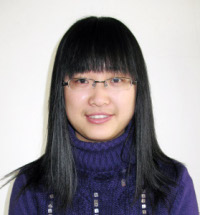
\includegraphics[height=4cm]{mypic.png}}
\begin{itemize}

\item {性别: }
女
\item {籍贯/出生年月: }
苏州/1984.07
\item {健康状况: }
良好
\item {政治面貌: }
中共党员
\item {毕业院校: }
\href{http://www.yzu.edu.cn}{扬州大学}, 信息工程学院
\item {专业及方向: }
管理科学与工程(Web搜索与Web挖掘)
\item {学历: }
硕士/2010年六月毕业
\item {通讯地址: }
江苏省扬州大学信息工程学院400173信箱(邮编:225009)

\end{itemize}

\resheading{教育经历}
\begin{itemize}

\item
    \ressubheading{硕士阶段}{}{2007年9月 - 现在}{}
    \begin{itemize}
        \resitem{   以优异成绩推荐免试于扬州大学信息工程学院,攻读管理科学与工程硕士学位.}
        \resitem{在校完成基础课程的学习,主要有: 计算机网络技术,最优化理论,人工智能,机器学习,数据仓库等,随后在上海交通大学进行访问学习,参与相关方向的研究工作,主要是关于文本与Web数据挖掘、 Web搜索相关方面的学习与研究,并参与项目团队的开发.目前已发表相关学术论文.}
    \end{itemize}
\item
    \ressubheading{本科阶段}{}{2003年9月 - 2007年7月}{}
    \begin{itemize}
        \resitem{   于扬州大学信息工程学院,攻读信息管理与信息工程专业学士学位.}
        \resitem{认真学习各门基础课程,主要有:高等数学,离散数学, 概率论与数理统计, 线性代数, C语言程序设计,C++程序设计,数据结构,操作系统原理,编译原理,数据库原理及应用,面向对象技术,计算机网络,软件工程, 人工智能,微机原理等,并取得优异成绩.}
    \end{itemize}

\end{itemize}

\resheading{技能及相关证书}
\begin{itemize}
\item{语言:}
熟悉Java、C/C++;
\item{Web技术:}
熟悉Web应用开发; 熟练掌握Html,CSS,Javascript等Web技术,并熟练使用
JQuery,并有Ajax、Servlet开发经验;
\item{数据库技术:}
熟悉使用Access数据库、SQL Server、MySQL;
\item{英语水平:}
CET-6
\item{计算机水平:}
获国家计算机等级考试三级优秀;

\end{itemize}

\resheading{项目经历}
\begin{itemize}

\item
    \ressubheading{建立校园网Web搜索服务平台}{}{2007.9~2007.12}{}
    \begin{itemize}
        \resitem{   描述: 校园网上的信息资源繁杂,为能够快速有效的找到相关信息,该项目在校园网上搭建一个提供搜索服务的平台,即建立一个基于校园网的Web搜索引擎,它可以将分散在各个应用系统和服务器上的信息进行过滤、整合和排序然后作为搜索结果返回.}
        \resitem{   职责: 主要包括:编写网络爬虫抓取整个校园网上的所有网页,存储并进行索引。搜索结果优化及用户接口设计。其中网络爬虫主要使用Java语言编写,使用Lucene开源工具包建立索引,并采用PageRank算法优化搜索结果。在Mvc框架下,采用JS+Servlet前后台Web技术设计用户接口,建立了一个高效的搜索引擎。}
    \end{itemize}

\item
    \ressubheading{大规模类别体系下的网页分类评测与算法研究}{}{2008.11~现在}{}
    \begin{itemize}
        \resitem{   描述: 当前,大规模类别体系下的网页自动分类技术在网页主题分析、搜索结果聚类、个性化信息检索、个性化网页、搜索引擎的目录导航服务、信息过滤、主动信息推送服务/广告配送,舆情监控,产品/商业信息分类等领域都有广泛的应用前景和商业运用价值.然而在大规模类别体系下的分类未取得令人满意的效果,因此,它是一个非常值得深入研究的领域.}
        \resitem{   职责: 阅读大量国内外学术论文,研究各种分类算法及其分类效率和分类效果,分析大规模类别体系下的分类存在的缺陷和难点,提出了大量新颖的方法和策略.包括使用梯度渐进的迭代思想、分类器的组合(不同类型分类器的集成)、可视化结果分析、分类算法的创新应用以及在解决大规模类别体系下分类算法遇到的问题与算法评测中也使用了创新方法和思想.并进行国家自然科学基金的申报,最后发表系列论文.}
    \end{itemize}

\item
    \ressubheading{C2C电子商务统计分析平台的构建}{}{2009.6~现在}{}
    \begin{itemize}
        \resitem{   描述: 此项目是建立C2C免费电子商务统计平台,现在主要是针对淘宝网、拍拍网还有百度的有啊网上的海量数据进行统计分析与预测,包括商品的分类统计、店铺统计地区统计,商品搜索以及TOP 50的分类统计等.采用Python编写的网络爬虫通过一定的爬取和更新策略和方法获得尽可能全而快的海量数据,采用8个服务器搭建的Hadoop平台上进行数据的处理、分析、统计,以及用Hbase进行数据存储的.其网址http://www.c2ctongji.com. }
        \resitem{   职责: 主要负责需求分析,整体架构设计,具体在Hadoop平台上进行分布式网页索引,还包括前台的js设计,主要用到的技术有:JQeury、Ajax、Servlet.}
    \end{itemize}

\item
    \ressubheading{其他完成的Demo}{}{2008.10 - 2008.11}{}
    \begin{itemize}
        \resitem{   中文搜索聚合系统,该系统聚合多个搜索引擎的返回结果,为用户提供一站式访问接口.系统提供的服务包括网页,问答、图片、视频、百科、商品、博客等多个优质搜索的结果.网址为:http://searchmash.apexlab.org }
        \resitem{   中文搜索反馈系统,SearchFeed 该系统聚合百度与Google的搜索引擎结果,用户在使用本系统后会提供用户使用该查询的所有反馈信息.网址为:http://searchfeed.apexlab.org}
    \end{itemize}

\end{itemize}

\resheading{发表论文}

\begin{itemize}
\item{2009 }
一种基于排序学习的查询意图预测算法
\item{2009 }
基于类别层次体系的商品分类研究
\item{2009 }
一种商品标题主题词的重要性排序算法
\item{2008 }
基于Lucene的校园网Web搜索服务研究与实现

\end{itemize}

\resheading{奖励/证书}
\begin{itemize}

\item{2003 - 2004学年 }
获三等专业奖学金;
\item{2004 - 2005学年 }
获二等专业奖学金;
\item{2004 - 2005学年 }
被评为校"优秀共青团员";
\item{2005 - 2006学年 }
获校二等奖学金;
\item{2005 - 2006学年 }
被评为校"三好学生";
\item{2007学年 }
获"优秀毕业生"称号;

\end{itemize}

\end{document}
